%!TEX root = ../main.tex
\documentclass[float=false, crop=false]{standalone}
\usepackage[subpreambles=true]{standalone}

\begin{document}

\section{Results and Research Products}
% Experiment 1 investigates CBF guidance display benefits (will be complete)
% Experiment 2 uses simulation of robotic arm
% Compare subjects with and without feedback in a track and capture task
% We can use this to validate the results we find in following experiment
% We can also use this to create our model and validate the predictions of the model

\subsection{Experiment 1}
Experiment One investigated the effects of concurrent bandwidth feedback on performance in a three-axis manual tracking task.
%
% Two pages of task description, methodology, analysis and results from AIAA submission.
%
% For this study we chose a common type of secondary task, the choice reaction time task.
% In this secondary task, subjects are presented with several different stimuli, each of which requires a different response~\cite{lysaght1989operator}.
% Subjects' objective workload can then be inferred by either the percentage of secondary tasks which were correctly responded to within a given time, the number of secondary tasks which were correctly responded to in a trial, or both.
% We have previously found this type of task to be accurately tied to subjective workload scales~\cite{Karasinski2017}.
%
%
% \subsubsection{Materials and Method}
% \begin{figure}[b!]
%     \begin{center}
%         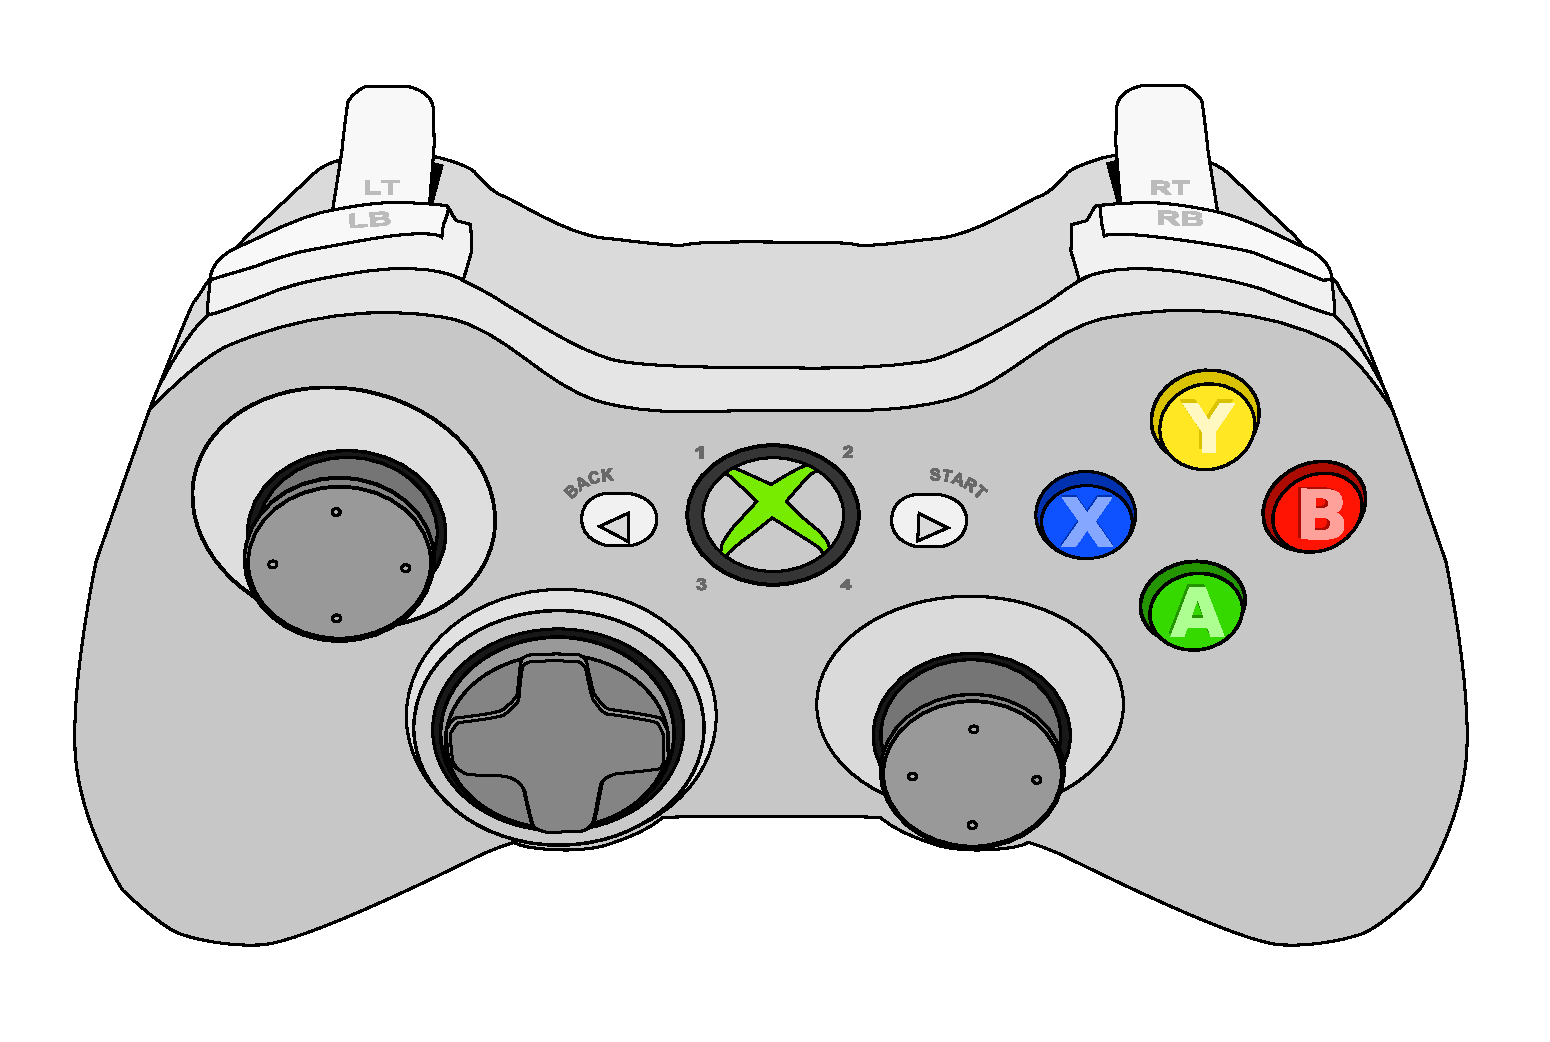
\includegraphics[width=0.5\linewidth]{../img/Xbox_Controller.pdf}
%         \caption{The Microsoft Xbox controller that subjects used to complete the task.}%
%         \label{fig:controller}%
%     \end{center}
% \end{figure}
In our experiment, subjects were responsible for simultaneously completing three tracking tasks and a two-choice task.
Each axis of the tracking task was disturbed by a sum-of-sines, resulting in a random appearing signal that was difficult for the subjects to predict.
The two-choice task appeared on a screen next to the tracking task, and asked subjects to respond to either a ``LEFT'' or ``RIGHT'' command.
Subjects controlled the three-axes and responded to the two-choice task by using a Microsoft Xbox controller.
The subjects used the left axis of the controller to control the $x$ and $y$ axes tracking tasks.
Subjects moved this controller left and right to control the $x$ axis, and up and down to control the $y$ axis.
The subjects used the right axis of the controller to control the $z$ axis.
Subjects moved this controller up and down to control the $z$ axis.
Subjects used the left and right triggers on the controller to respond to the two-choice task, using the left trigger to indicate ``LEFT'' on the two-choice task, and the right trigger to indicate ``RIGHT'' on the two-choice task.

\subsubsection{Stereoscopic Displays}
Stereoscopic displays are systems ``in which two slightly different views of a scene are provided to a viewer, one image for each eye... allow[ing] the viewer's binocular visual system to extract depth information in a scene using this disparate information''~\cite{McIntire2014}.
Without the aid of the binocular depth cue presented by stereoscopic displays, viewers are instead reliant entirely on monocular clues such relative sizing, occlusion, and motion.
One of the primary motivation for stereoscopic displays is that ``[t]he visual scene of a 3D world is a more `natural,' `ecological,' or `compatible' representation than that provided by 2D displays''~\cite{Wickens1990}.
As a result of this motivation, the effects of stereoscopic displays on human performance have been extensively studied in the literature.
Several authors have attempted to classify which types of tasks may stand to benefit~\cite{McIntire2014, Wickens1990, Wickens1989, Naikar1998, Dixon2009}.
A recent review of 184 papers, for example, suggests that 60\% of studies showed some benefit of 3D stereo displays, 15\% of tasks showed unclear or mixed benefits, and 25\% of studies showed no clear benefits~\cite{McIntire2014}.
In this study, tasks involving finding/identifying/classifying objects and tasks involving real/virtual spatial manipulations of objects benefited the most, while learning/training/planning tasks were the least likely to show a benefit.

Kim et al. also performed a quantitative evaluation of perspective and stereoscopic displays in three-axis manual tracking task~\cite{Kim1987}.
They investigated the differences between perspective and stereoscopic displays, the elevation angle, azimuth angle, and the effects of two visual enhancements: a grid and a reference line.
They found very strong relationships between elevation and azimuth angles and tracking performance, with the best performance occurring with an elevation angle of 45 degrees and an azimuth angle of 0 degrees.
Tracking performance decreased rapidly as the azimuth angle varied, and decreased less rapidly as the elevation angle varied.
In generally, they found that the stereoscopic display allowed for better tracking performance, though the inclusion of the reference line visual enhancement greatly decreased the benefit over the perspective display.
Using only two subjects, they provided some insight into intrasubject and intersubject variability.
In several instances, intrasubject variability showed 50\% changes within the same experimental condition, while intersubject variability also appeared to be large in some conditions.
Kim et al. repeated the evaluation of these parameters on a telerobotics pick and place study~\cite{WonKim1987}.
They found similar results in this second study, suggesting that their results could be generalized and that three-axis tracking performance can be correlated with pick and place completion time.

Smallman at al. similarly investigated the effect of visual enhancements and 2D vs 3D displays for the development of a naval air warfare console~\cite{Smallman2000}.
Participants viewed naval and aircraft tracks in either a conventional 2D top-down display or a 3D display, and then attempted to reconstruct track positions.
They investigated the effectiveness of drop-lines and drop-shadows, and found that they significantly improved subjects ability to localize aircraft compared to when the enhancements were not present.
Furthermore, in the absence of either visual enhancement subjects performed better with the 2D display than the 3D display.
Similar to Kim et al., they ultimately recommended that 3D stereoscopic displays include the use of a reference or drop-line for optimal performance.


\subsubsection{Hypotheses}
This study assessed the influence of display (perspective vs. stereoscopic), relative display attitude (zero degrees vs. thirty degrees), and concurrent bandwidth feedback (with vs. without) on performance and workload.
Objective performance was measured using the root-mean-square error (RMSE) of each of the three axes individually and combined, and subjective performance was measured with the use of a questionnaire.
Objective workload was measured using the response time to the secondary task, and subjective workload was measured using the NASA-TLX.
It is hypothesized that:
\begin{description}[align=left]
\item [Hypothesis 1] Concurrent bandwidth feedback will improve performance in the depth ($z$) axis for both display types, and will decrease workload.
\item [Hypothesis 2] Stereoscopic augmented reality displays improve performance in the depth ($z$) axis, but do not affect workload.
\item [Hypothesis 3] Rotating the display improves performance in the depth ($z$) axis for both display types, and will decrease workload.
% \item [Hypothesis 4] The performance along the $x$ and $y$ axes will be the same for all three designs.
\end{description}

\subsubsection{Procedure}
% \subsubsection{Participants}
A total of 24 subjects (19 males, 5 females) were recruited in accordance with the University of California, Davis Internal Review Board (IRB).
There were 12 subjects in the LCD group, and 12 subjects in the HoloLens group.
Subjects were undergraduate and graduate students in the University of California, Davis College of Engineering.
%, and had a mean age of $XX \pm XX$.
This experiment was approved by the Institutional Review Board at the University of California, Davis, and subjects signed a consent form and were not compensated.

% \subsubsection{Apparatus}
\begin{figure}[tb!]
    \begin{center}
        \begin{subfigure}{0.49\textwidth}
            \includegraphics[width=\linewidth]{../img/DSC_0801.JPG}
            \caption{LCD Group}
        \end{subfigure}\hfill
        \begin{subfigure}{0.49\textwidth}
            \includegraphics[width=\linewidth]{../img/DSC_0803.JPG}
            \caption{HoloLens Group}
        \end{subfigure}
    \caption{The fixed-based simulator used by both groups.}%
    \label{fig:simulator}%
    \end{center}
\end{figure}

% \paragraph{Equipment}
A human-in-the-loop simulation was conducted using a fixed-base simulator, see Figure~\ref{fig:simulator}.
The simulator consisted of two 10.4 inch LCD displays.
The tracking task was completed on the left display, while the right display showed the two-choice task.
Subjects were seated for the duration of the experiment, and were placed one meter perpendicular from the center of the left display.
For subjects in the HoloLens group, the left LCD monitor was turned off, and the tracking task was instead displayed on the HoloLens.
For these subjects, the cross was placed at the same height as the subject's head, such that it was viewed directly on in the baseline condition.
% different height subjects -> tracking cross was at different heights
% no way to avoid this AND keep the relative view angle the same between groups
% The cross was rendered at 800x480 pixels for the LCD group, and at 1268x720 pixels for the HoloLens group.
Both groups, however, viewed the guidance cross of a width and height of 5 inches by 5 inches.
For subjects in the HoloLen's group, the $z$ motion of the cross also could move up to 5 inches in either direction away from the center of the guidance cross.
Subjects in both groups used the same Microsoft Xbox controller to complete the task.

% \paragraph{Selection of Disturbance}
The disturbance function was a sum of 13 sinusoids approximating a rectangular spectrum with a 2.0 rad/s cutoff frequency~\cite{hess1984effects}.
The disturbing force, as a function of time, $d(t)$, was
\begin{align}
d(t) = \sum_{i=1}^{13} A_i \sin \left( w_i t + \phi_i \right)
\label{eq:disturbance}
\end{align}
Table~\ref{sine-table} lists the sine wave amplitude, frequency, number of cycles in a 60 second run, and phase offset for each sine wave in the disturbance force.
This disturbance was the same for all subjects and trials, though the subjects were naive to this.
The $x$, $y$ and $z$ axes all experienced the same disturbance force generating function, but the $y$ axis was temporally offset by 60 seconds and the $z$ axis was offset by 120 seconds.
This allowed for a very similar generation of disturbance forces for each axis.
The RMSE of the disturbance force was normalized along each axis such that all three were the same.

\begin{table}[tb]
\caption{The relative amplitude, frequency, number of cycles in each 60 second run, and phase offset each $i^{th}$ sine, see Equation~\ref{eq:disturbance}.}
\centering
\begin{tabular}{*{5}{r}}
\toprule
i & $A_i/A_1$ & $w_i$ rad/s & \multicolumn{1}{p{3cm}}{\centering No. of cycles \\in 60-s run} & $\phi_i$ \\
\midrule
1  & 1.0 &  0.18850 & 1   & $\pi/6.5$ \\
2  & 1.0 &  0.31416 & 3   & $2 \times \phi_1$ \\
3  & 1.0 &  0.50265 & 4   & $3 \times \phi_1$ \\
4  & 1.0 &  0.87965 & 8   & $4 \times \phi_1$ \\
5  & 1.0 &  1.44513 & 13  & $5 \times \phi_1$ \\
6  & 1.0 &  2.13628 & 20  & $6 \times \phi_1$ \\
7  & 0.1 &  3.07876 & 29  & $7 \times \phi_1$ \\
8  & 0.1 &  4.20973 & 40  & $8 \times \phi_1$ \\
9  & 0.1 &  5.78053 & 55  & $9 \times \phi_1$ \\
10 & 0.1 &  8.23097 & 78  & $10 \times \phi_1$ \\
11 & 0.1 & 11.24690 & 107 & $11 \times \phi_1$ \\
12 & 0.1 & 15.77079 & 150 & $12 \times \phi_1$ \\
13 & 0.1 & 23.93894 & 228 & $13 \times \phi_1$ \\
\bottomrule
\end{tabular}
\label{sine-table}
\end{table}

% \paragraph{The Three Designs}
\begin{figure}[tb!]
    \begin{center}
        \begin{subfigure}{0.32\textwidth}
            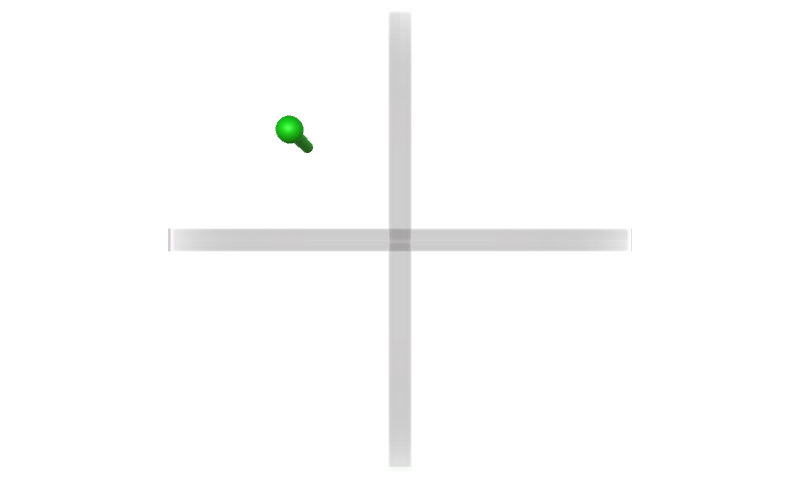
\includegraphics[trim={5cm 0 5cm 0},clip,width=\linewidth]{../img/Baseline.png}
            \caption{Baseline}
        \end{subfigure}\hfill
        \begin{subfigure}{0.32\textwidth}
            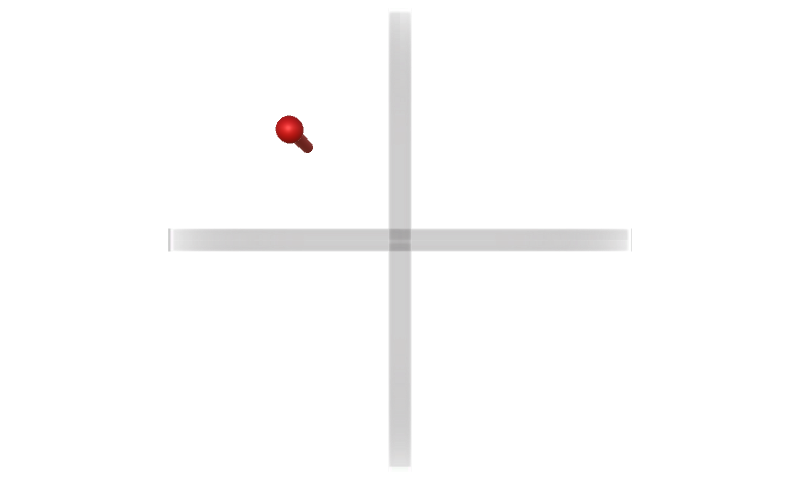
\includegraphics[trim={5cm 0 5cm 0},clip,width=\linewidth]{../img/Color.png}
            \caption{Color}
        \end{subfigure}\hfill
        \begin{subfigure}{0.32\textwidth}
            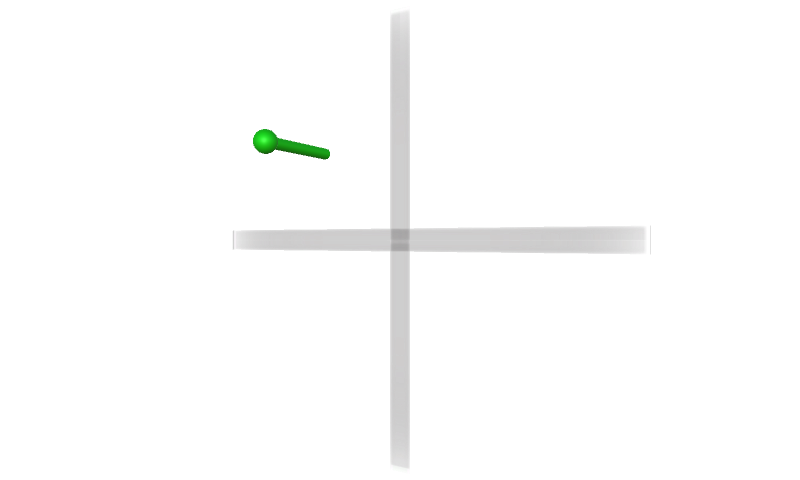
\includegraphics[trim={5cm 0 5cm 0},clip,width=\linewidth]{../img/Angled.png}
            \caption{Rotated}
        \end{subfigure}
        \caption{The three different designs in the same error state.
        (b) The color feedback has been activated here, changing the guidance target from green to red.}
        \label{fig:designs}%
    \end{center}
\end{figure}

\begin{figure}[tb!]
    \begin{center}
        % Thanks
        % https://tex.stackexchange.com/questions/67573/tikz-shift-and-rotate-in-3d

        \newcommand{\rotateRPY}[3]% roll, pitch, yaw
        {   \pgfmathsetmacro{\rollangle}{#1}
            \pgfmathsetmacro{\pitchangle}{#2}
            \pgfmathsetmacro{\yawangle}{#3}

            % to what vector is the x unit vector transformed, and which 2D vector is this?
            \pgfmathsetmacro{\newxx}{cos(\yawangle)*cos(\pitchangle)}
            \pgfmathsetmacro{\newxy}{sin(\yawangle)*cos(\pitchangle)}
            \pgfmathsetmacro{\newxz}{-sin(\pitchangle)}
            \path (\newxx,\newxy,\newxz);
            \pgfgetlastxy{\nxx}{\nxy};

            % to what vector is the y unit vector transformed, and which 2D vector is this?
            \pgfmathsetmacro{\newyx}{cos(\yawangle)*sin(\pitchangle)*sin(\rollangle)-sin(\yawangle)*cos(\rollangle)}
            \pgfmathsetmacro{\newyy}{sin(\yawangle)*sin(\pitchangle)*sin(\rollangle)+ cos(\yawangle)*cos(\rollangle)}
            \pgfmathsetmacro{\newyz}{cos(\pitchangle)*sin(\rollangle)}
            \path (\newyx,\newyy,\newyz);
            \pgfgetlastxy{\nyx}{\nyy};

            % to what vector is the z unit vector transformed, and which 2D vector is this?
            \pgfmathsetmacro{\newzx}{cos(\yawangle)*sin(\pitchangle)*cos(\rollangle)+ sin(\yawangle)*sin(\rollangle)}
            \pgfmathsetmacro{\newzy}{sin(\yawangle)*sin(\pitchangle)*cos(\rollangle)-cos(\yawangle)*sin(\rollangle)}
            \pgfmathsetmacro{\newzz}{cos(\pitchangle)*cos(\rollangle)}
            \path (\newzx,\newzy,\newzz);
            \pgfgetlastxy{\nzx}{\nzy};
        }

        \tikzset{RPY/.style={x={(\nxx,\nxy)},y={(\nyx,\nyy)},z={(\nzx,\nzy)}}}

        \begin{tikzpicture}
            \draw[-] node at (3.5,0,0) {x} (-3,0,0) -- (3,0,0);
            \draw[-] node at (0,3.5,0) {y, {\color{red} y\textprime}} (0,-3,0) -- (0,3,0);
            \draw[-] node at (0,0,3.5) {z} (0,0,-3) -- (0,0,3);

            \rotateRPY{0}{-30}{0}
            \begin{scope}[draw=red, text=red,fill=red,densely dashed,RPY]
                \draw[-] node at (3.5,0,0) {x\textprime} (-3,0,0) -- (3,0,0);
                %\draw[-] node at (0,3.5,0) {} (0,0,0) -- (0,3,0);
                \draw[-] node at (0,0,3.5) {z\textprime} (0,0,-3) -- (0,0,3);
            \end{scope}
            \draw [->] (0:1.5) arc (0:-15:1.5);
            \draw[-] node at (1.7,-.2,0) {$\theta$};
        \end{tikzpicture}

        \caption{Perspective display of the coordinate frame for the tracking tasks, with the $x$, $y$, and $z$ axes labeled. After rotating by $\theta$ around the y axis, the resulting reference frame of $x\textprime y\textprime z\textprime$ is also labeled.}
    \end{center}
\end{figure}

\begin{table}[tb]
\caption{The factors that were modified between the different designs.}
\centering
\begin{tabular}{*{3}{r}}
\toprule
Design & $\theta$ (degrees) & Feedback \\
\midrule
Baseline & 0 & No \\
Feedback & 0 & Yes \\
Rotated & 30 & No \\
\bottomrule
\end{tabular}
\label{tab:designs}
\end{table}

Three designs were presented to the subjects to evaluate: a baseline display, a color feedback display, and an rotated display.
Figure~\ref{fig:designs} shows all three designs in the same error state.
The three designs were very similar, having only minor differences between each other.
Compared to the baseline, the color feedback and rotated displays were expected to produce superior performance along the $z$ axis.

The baseline display consists of a flat cross which a center target point and a green sphere error indicator.
This indicator also casts a green rod perpendicular to the plane of the cross, which allows for a visual estimation of the error in the $z$ axis.
The $x$ axis is parallel with the horizontal cross, while the $y$ axis is parallel with the vertical cross.
The color feedback display was identical to the baseline design in every way, but also had visual concurrent bandwidth feedback on the $z$ axis.
When the absolute value of the error on the $z$ axis grew over a fixed bandwidth of 0.2 units, the color of both the spherical indicator and the cylindrical rod changed from green to red.
When the absolute value of the error on the $z$ axis was lowered back below this fixed bandwidth, the indicator changed back to a green color.
The rotated display was identical to the baseline design, but the relative attitude of the display was rotated about the $y$ axis by 30 degrees.

Before entering the study, subjects were randomly placed in a display group (either the LCD monitor or HoloLens), and were then randomly placed into an order group (which consisted of Baseline-Feedback-Rotated, Feedback-Rotated-Baseline, and Rotated-Baseline-Feedback).
This order group was created to remove any order effects that might arise due to training on a given display, and follows a standard latin squares design.
(The order of the designs was initially considered to be insignificant, but we will later discuss how this is not the case.)
% Subjects were naive to this order, and were only told which design they were evaluating directly before they began.
After entering the experiment room, the subjects signed a consent form, and then sat through a twenty minute training session which familiarized them with the task, the three designs, the NASA-TLX, and the controller.
Subjects were instructed that they were evaluating three different display designs: a baseline display, a color feedback display, and and rotated display.
They were further instructed that they had two tasks.
They were told to:
\begin{itemize}
    \item Minimize the displacement of your guidance target from the center
    \item Respond to the two choice task as accurately and quickly as possible
\end{itemize}

After the training, subjects were seated in front of the simulator.
Subjects in the HoloLens group then completed a short calibration program that adjusted the display to their interpupillary distance.
After this, they were instructed how to align the guidance cross with the center of the left display monitor.
All subjects were then allowed to complete two familiarization trials, during which time they could ask questions about how the controls worked, or any other aspects of the task.
The proctor also used this time to ensure that subjects had a basic grasp of the task, and were responding to both the tracking and two-choice tasks appropriately.
All familiarizations were done with the baseline design, regardless of which design the subjects evaluated first.

After this familiarization process, subjects completed ten trials in their first design.
Finishing this, they then completed a brief survey which asked them if the design was adequate to complete the task.
Subjects were also asked to subjectively rate their performance in a questionnaire after evaluating each design.
Subjects were asked ``I found the tracking display adequate to complete the task.'', and were asked to respond on a five point scale where 1 indicated ``Strongly Disagree'' and 5 indicated ``Strongly Agree''.
After this survey, subjects then completed a NASA-TLX workload survey
Subjects then repeated this process for their second and third designs.
After completing this process for their third design, subjects were also asked to complete a preference survey which inquired into what design the subjects believed to be the best.

\subsubsection{Results}
















\subsection{Experiment 2}
Experiment Two will investigate if concurrent bandwidth feedback can decrease the required learning time to peak performance in a simulated robotic arm pick and place task.
We will compare task performance and workload between two groups: a control group, which receives no feedback, and a treatment group, which receives concurrent bandwidth feedback on one or more sensor readouts.
Subjects in both groups will complete the same task, and it is hypothesized that subjects in the treatment group will perform the task better and require less training time to reach peak performance.
This hypothesis is based on the results of the SAFER experiment, as well as the results of Experiment One.

In this task, subjects will command a robotic arm to pick up an object from one location and place it in another.
This is analogous to the primary use of the robot arm on the International Space Station, which grasps visiting vehicles when they arrive at the station and then attaches them to a separate fixed location on the station.
Subjects will be trained on this task, and will then repeat the task for one to two hours through a variety of slightly different start and end conditions.
While they are completing the robotics task, subjects will also be required to attend to a secondary task which will require them to look away from their primary flight display.
Subjects will also be asked to report their subjective workload after each trial.

NASA’s Robotic Onboard Trainer (ROBoT) will be used for this experiment.
ROBoT is a package of simulation software which includes a dynamic model of the robotic arm on the space station, and presents the user with multiple camera angle views and the instrument panel required to operate effectively.
In addition to these displays, ROBoT also includes the two hand controllers required to control the arm.
NASA trainers at Johnson Space Center developed metrics which are included in ROBoT, and include the time to capture, alignment measurements during approach, the amount of wobble in the arm, the number of times the grapple fixture contacted the structure, the overall path efficiency, and the number of capture attempts.
This presents a list of candidate metrics from which we may observe human performance.

\begin{figure}[tb!]
    \begin{center}
        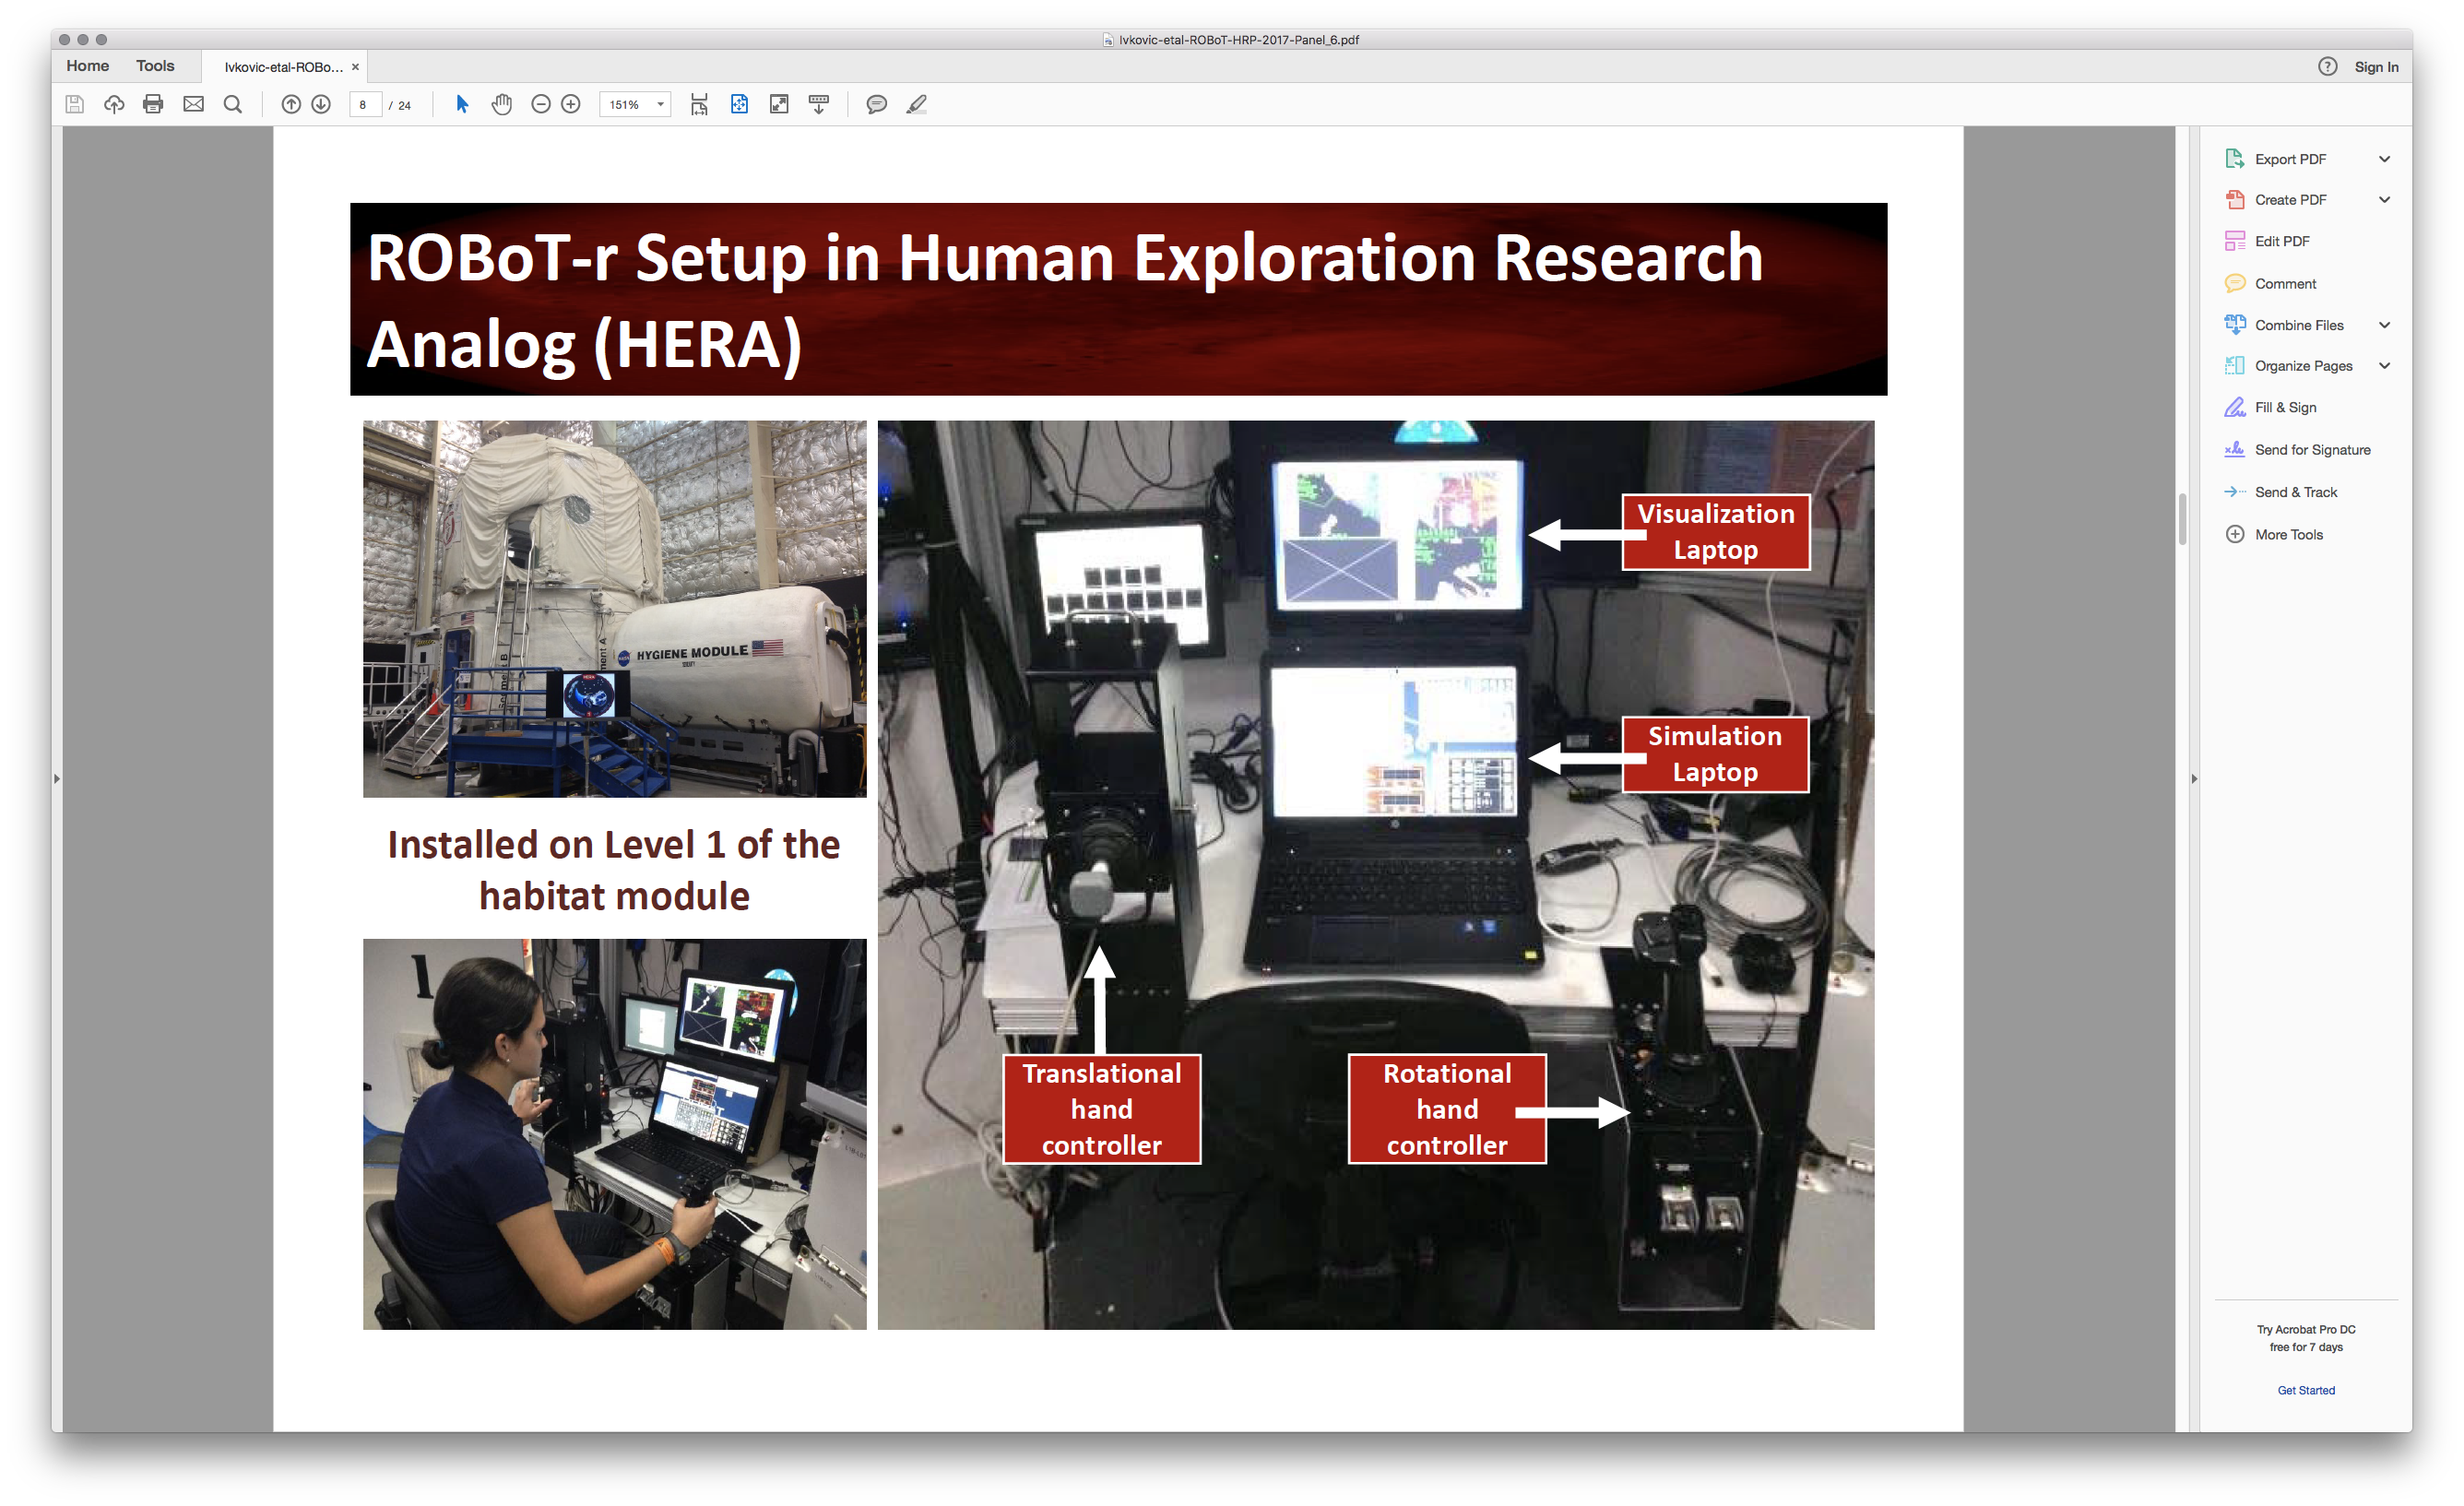
\includegraphics[trim={13cm 5cm 22cm 15.5cm},clip,width=\linewidth]{./../img/Screen Shot 2018-07-26 at 1.43.16 PM.png}
        \caption{The Robotic Onboard Trainer (ROBoT) station set up in the NASA HERA Analog.}
        % \label{}
    \end{center}
\end{figure}

\begin{figure}[tb!]
    \begin{center}
        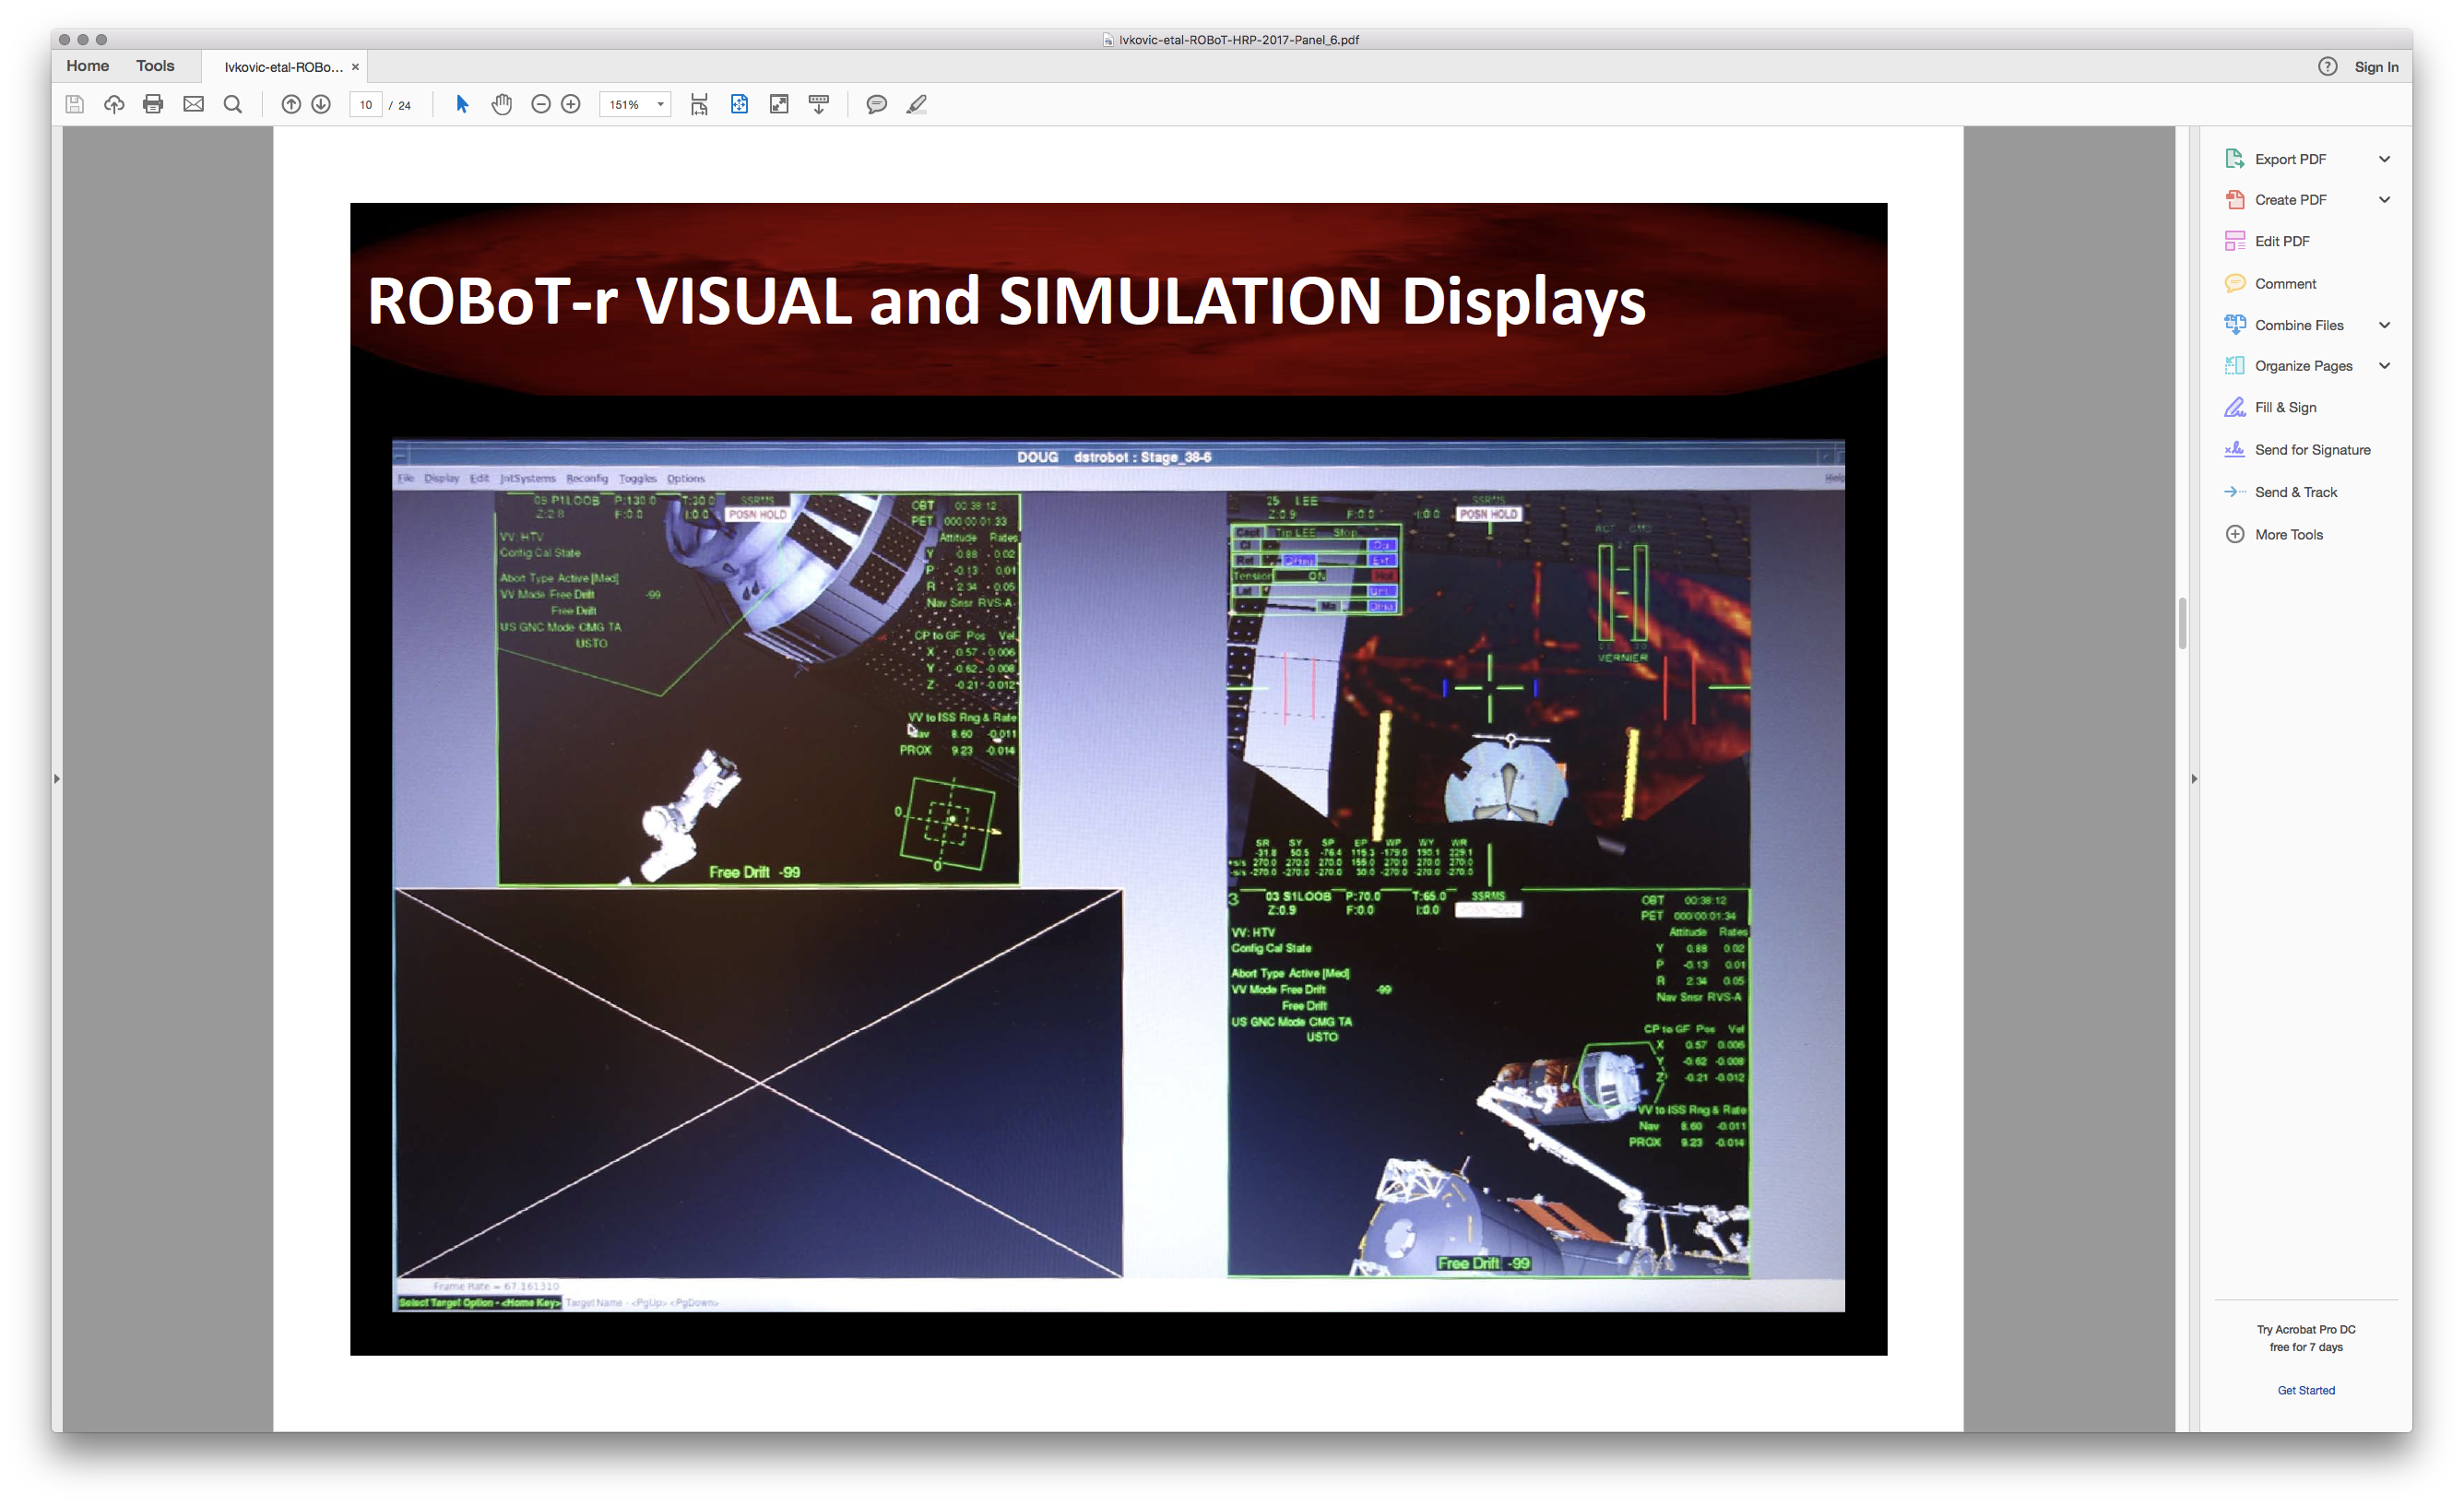
\includegraphics[trim={13cm 5cm 22cm 15.5cm},clip,width=\linewidth]{./../img/Screen Shot 2018-07-26 at 1.43.02 PM.png}
        \caption{ROBoT visualization laptop, showing four camera views.}
        % \label{}
    \end{center}
\end{figure}

\begin{figure}[tb!]
    \begin{center}
        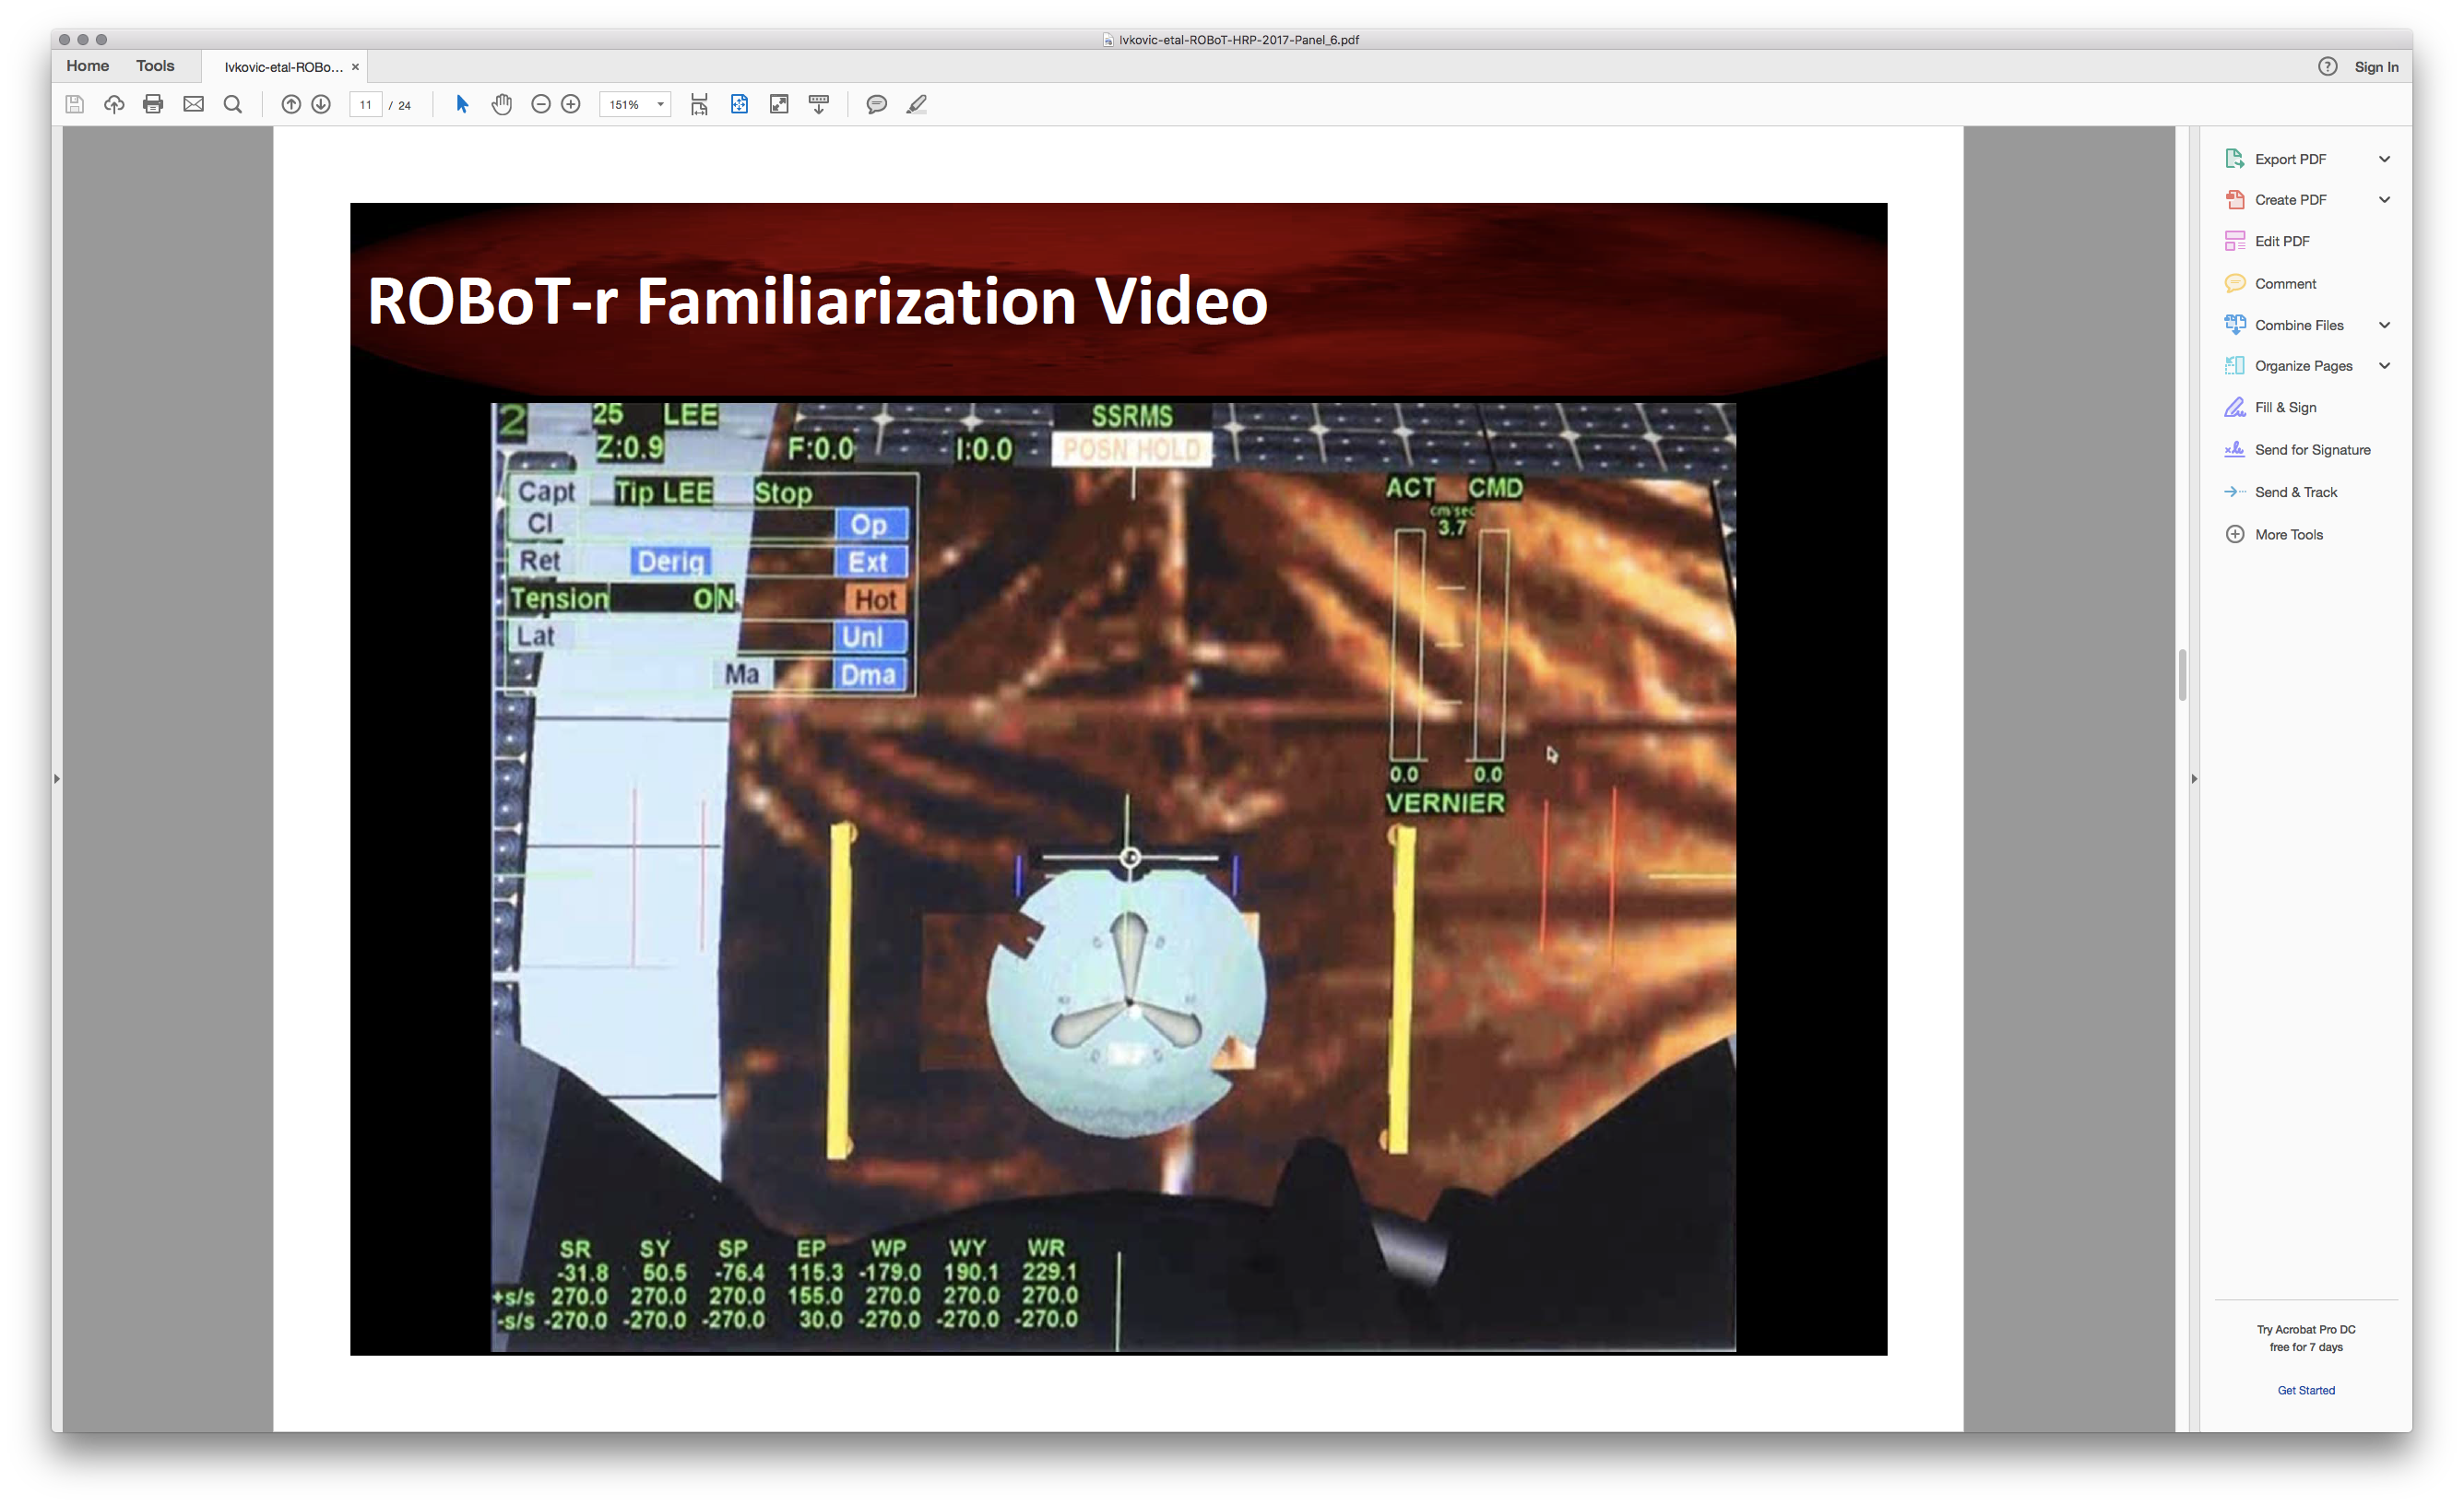
\includegraphics[trim={13cm 5cm 22cm 15.5cm},clip,width=\linewidth]{./../img/Screen Shot 2018-07-26 at 1.43.05 PM.png}
        \caption{The camera attached to the end effector of the robotic arm, showing the grapple fixture.}
        % \label{}
    \end{center}
\end{figure}

% \begin{figure}[tb!]
%     \begin{center}
%         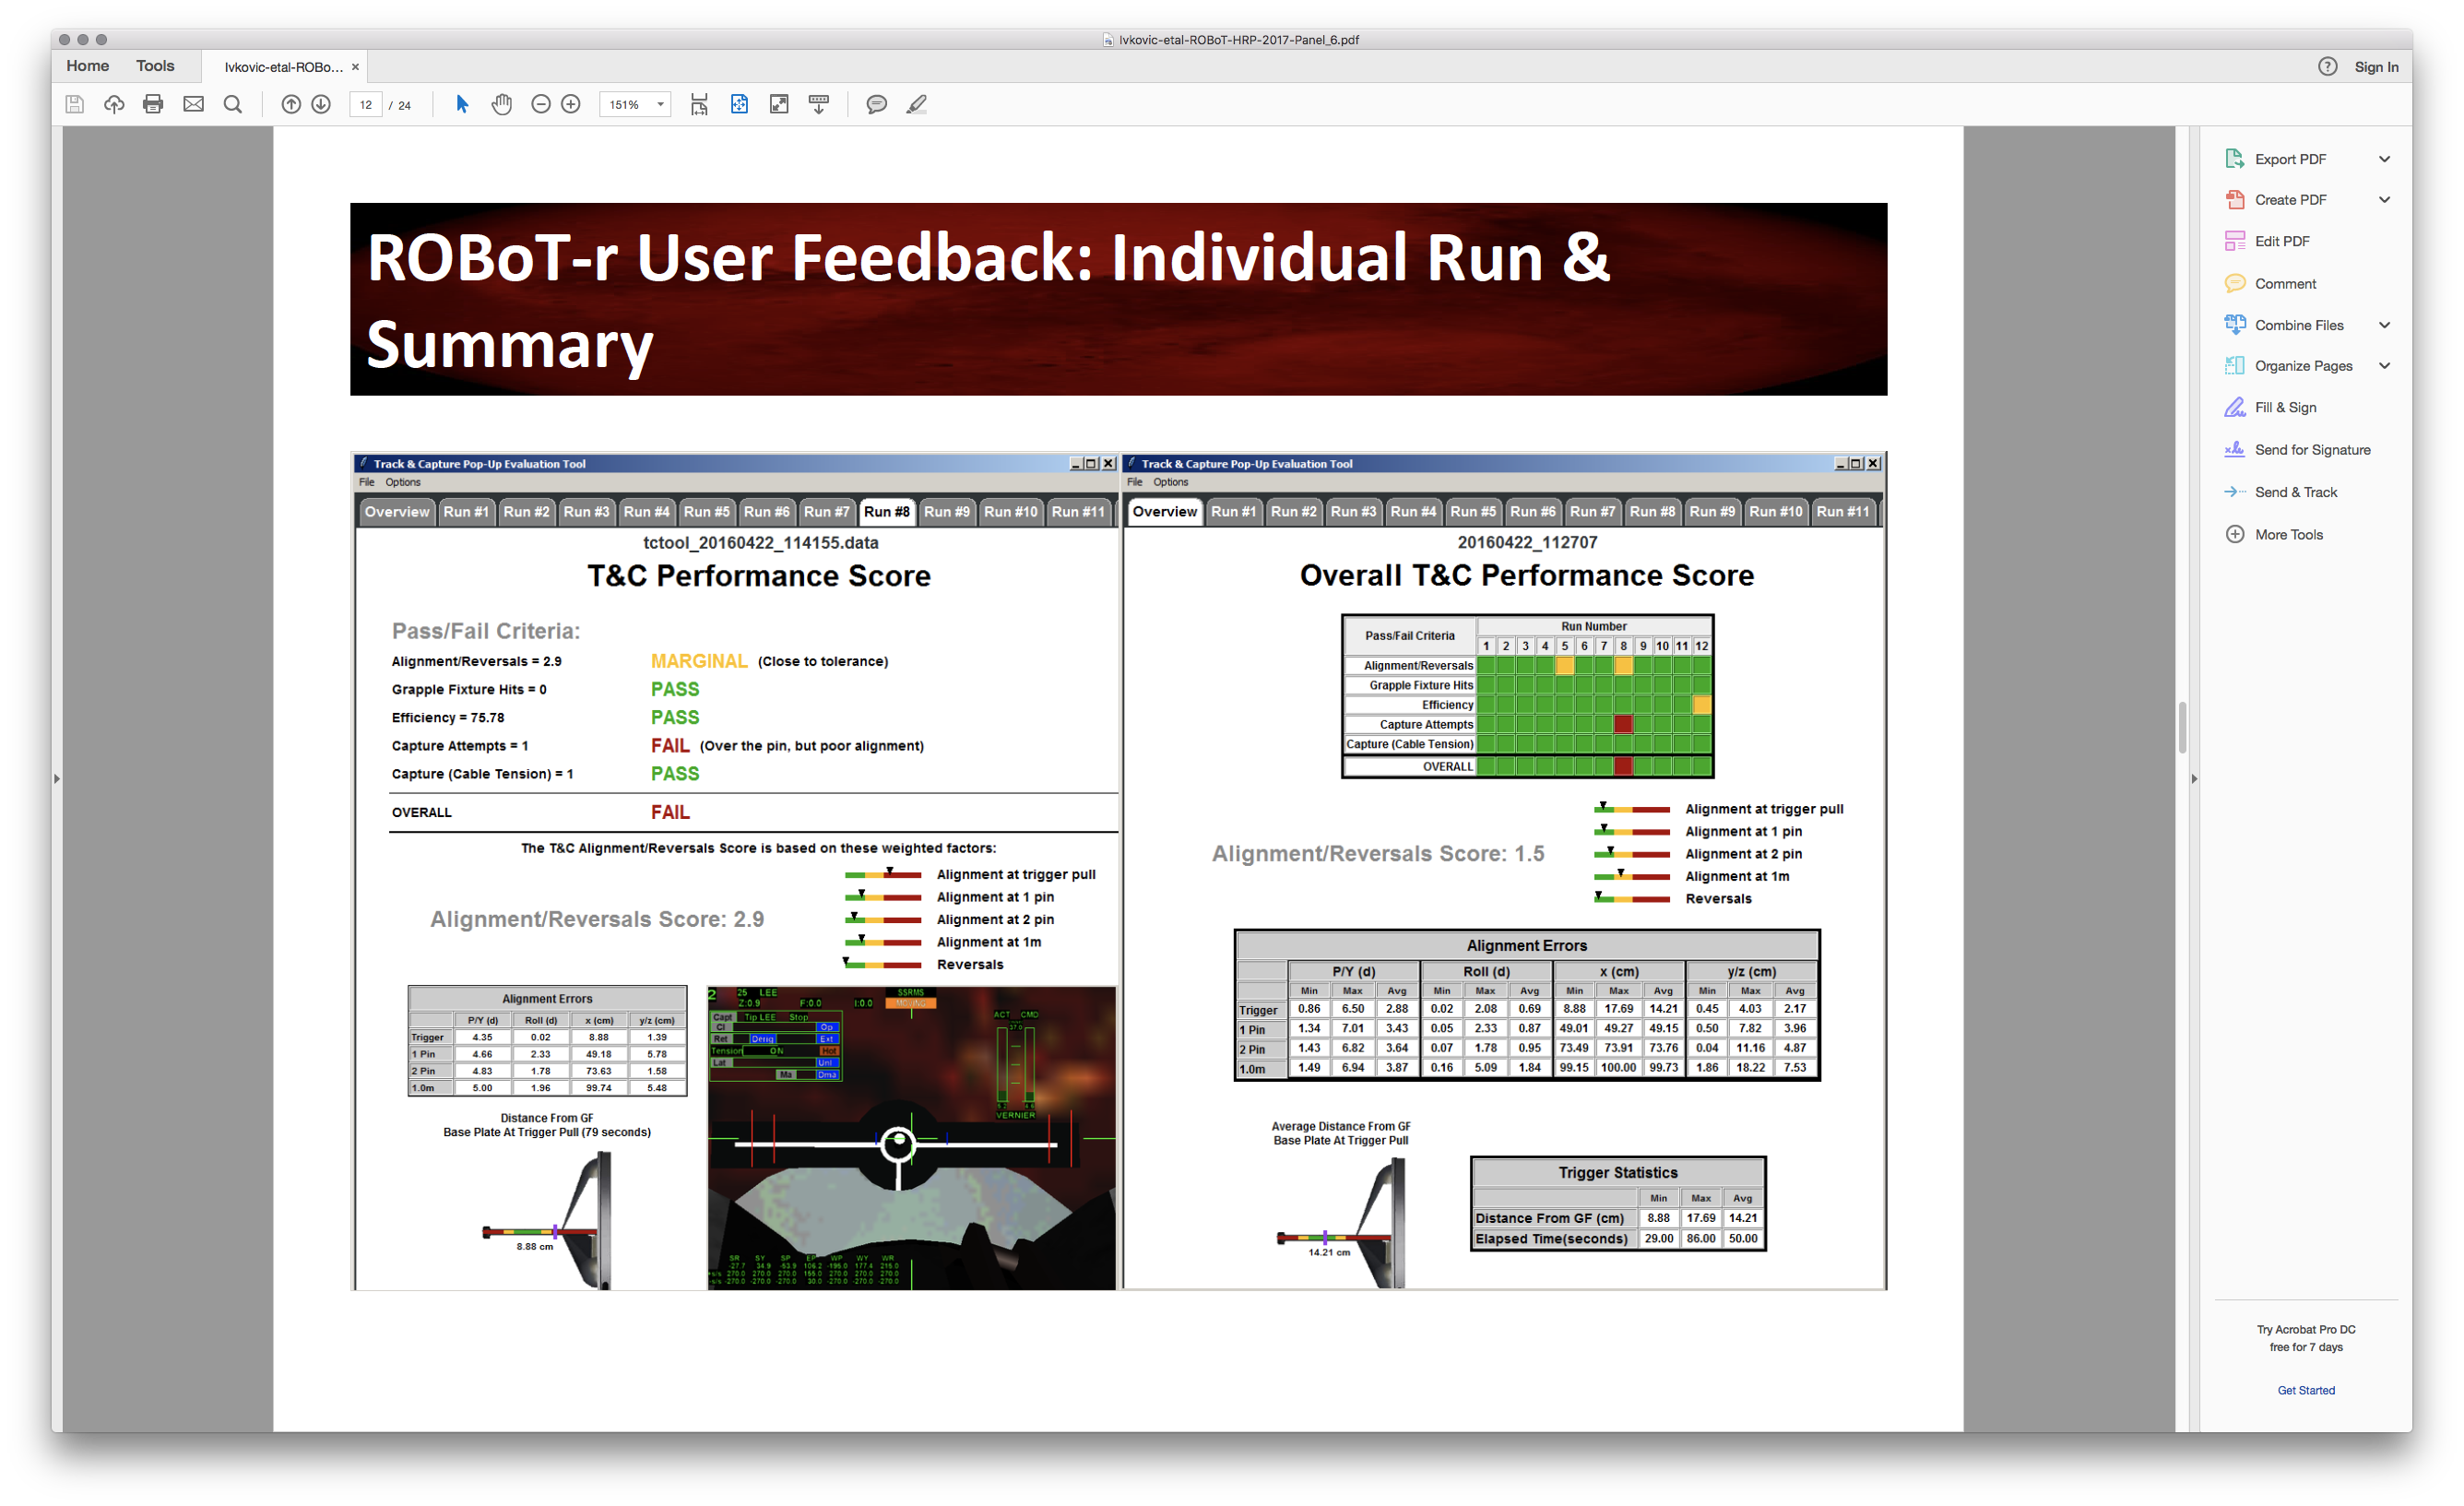
\includegraphics[trim={13cm 5cm 22cm 15.5cm},clip,width=\linewidth]{./../img/Screen Shot 2018-07-26 at 1.43.07 PM.png}
%         \caption{Example performance score report shown to the user after each trial.}
%         % \label{}
%     \end{center}
% \end{figure}

% \begin{figure}[tb!]
%     \begin{center}
%         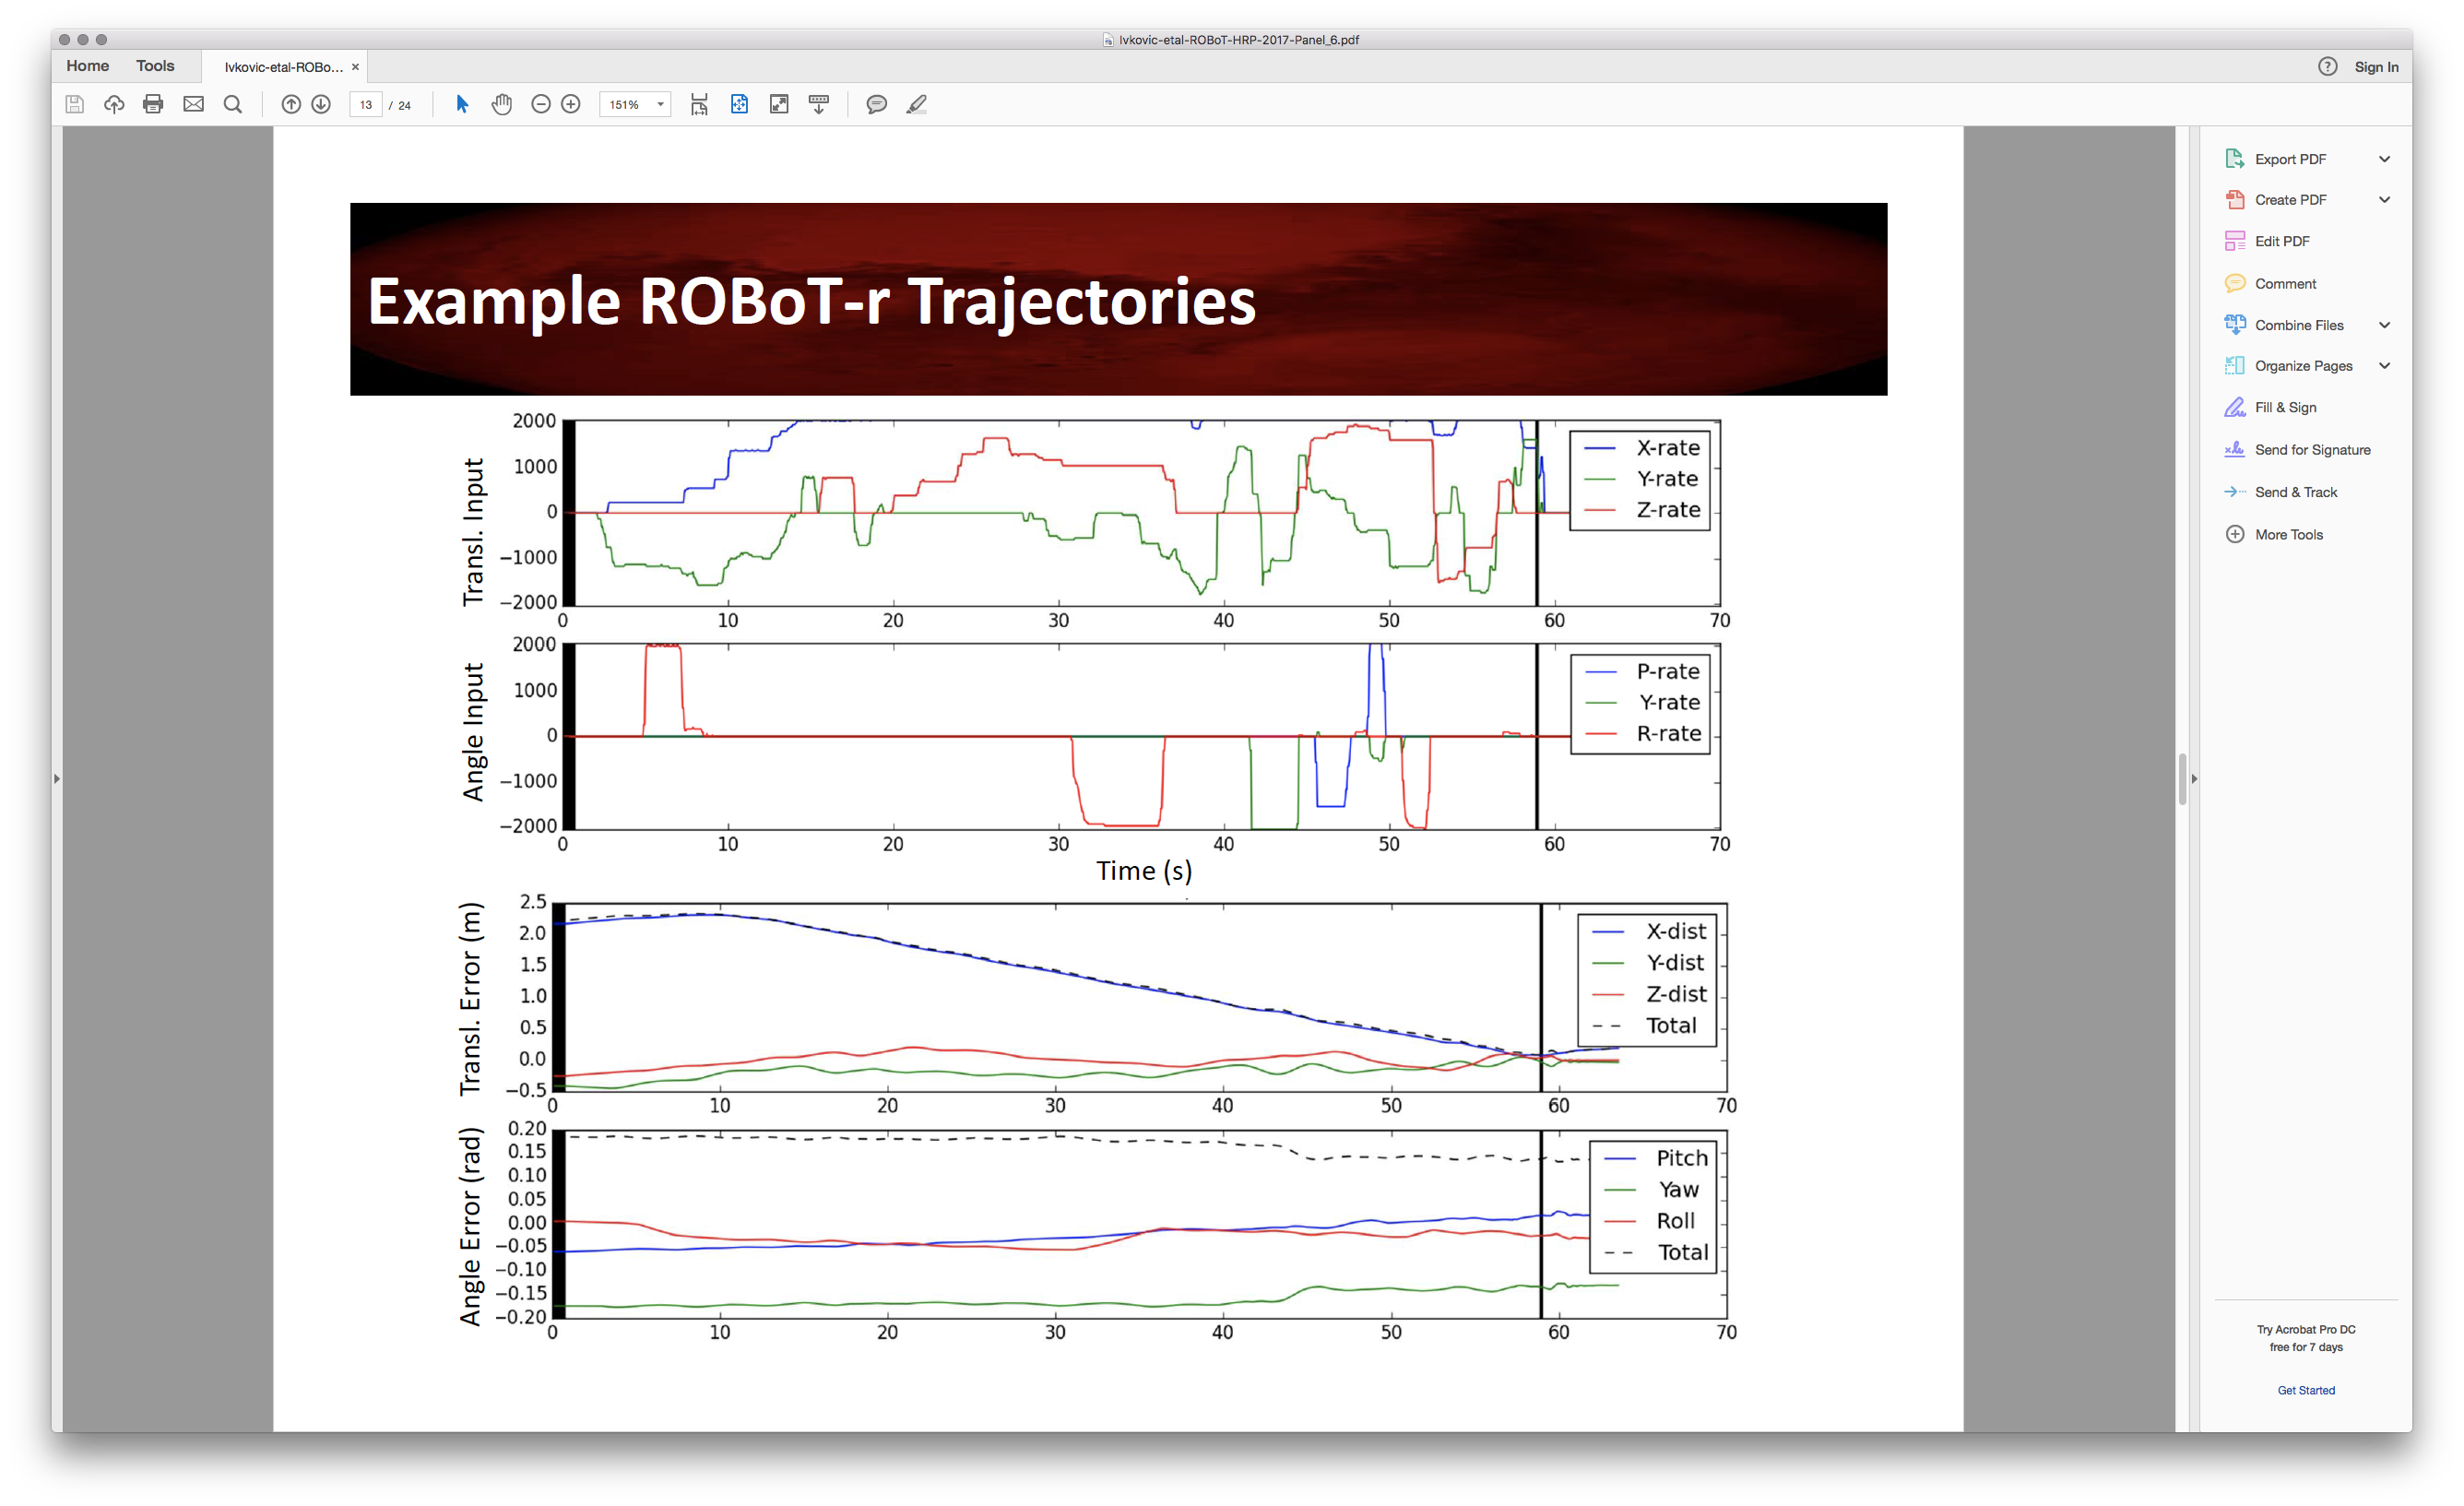
\includegraphics[trim={13cm 5cm 22cm 15.5cm},clip,width=\linewidth]{./../img/Screen Shot 2018-07-26 at 1.43.10 PM.png}
%         \caption{The hand controller inputs and position and angular errors are also logged throughout the trial.}
%         % \label{}
%     \end{center}
% \end{figure}


\subsection{Model Extension}
The Model will extend Professor Hess’ structural model of the human pilot to include the effects of concurrent bandwidth feedback.
The outputs of this model will be compared to the results of Experiment One and Two.

\subsection{Timeline}

\begin{figure}[h!]
    \begin{center}
        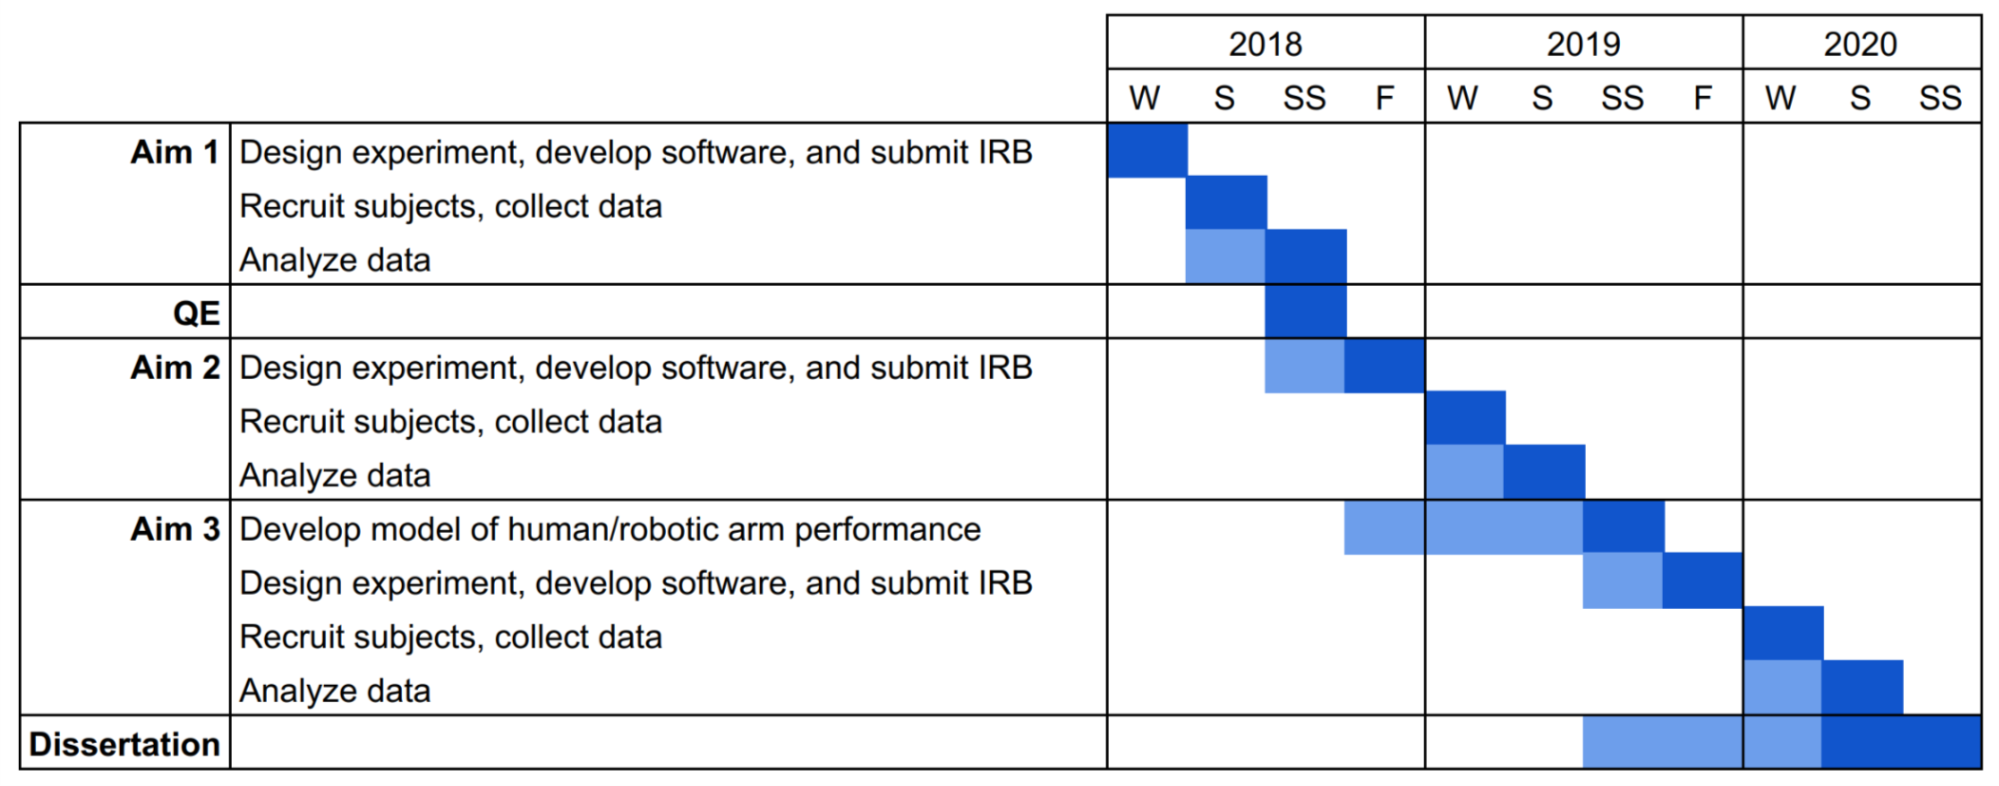
\includegraphics[width=\linewidth]{./../img/image1.png}
        % \caption{}
        % \label{}
    \end{center}
\end{figure}

\end{document}
